\clearpage
\section{Forschungsgrundlage}
\label{sec:research}

Um zu untersuchen, wem funktionale Programmierung Grundkenntnisse effektiver beibringen könnte als häufiger verwendete Paradigmen, muss zunächst die theoretische Grundlage gebaut werden. In diesem Abschnitt wird Computational Thinking exakt definiert, und auf vier häufigste Aspekte reduziert. Zudem wird das Lerntypenmodell, das in dieser Arbeit verwendet wird erläutert. Zum Schluss wird belegt, dass Objektorientierte und Prozedurale Programmierparadigmen tatsächlich häufiger in Einführungskursen der Informatik verwendet wird, als funktionale Programmierung.

\subsection{Computational Thinking}

\subsubsection{Definition}
Der Begriff Computational Thinking (CT) wurde erstmals 1980 verwendet \cite{papert}, schlussendlich allerdings erst 2006 wieder weitläufig durch eine Kolumne in den öffentlichen Diskurs gebracht \cite{wing2006}.
Grund der erneuten popularisierung des Begriffes war unter anderem die Diskussion von CT in Kontext von Schulcurricula, und die Wichtigkeit des Konzeptes im Alltag.
Aufgrund dessen, dass es keine allgemein akzeptierte, einheitliche Definition des CT gibt, wurden sich im Kontext der Arbeit verschiedenste Studien betrachtet und verglichen. Es wurde sich für einheitliche Definitionen an einer Review Studie aus dem Jahre 2017 orientiert, die bisherige Forschungsergebnisse abwägt und vergleicht \cite{schute}.
\\
In den frühesten Definitionen von CT wird das Konzept häufig beschrieben als Grundlage für alle unsere Prozesse im Alltag. CT ist demnach nicht nur eine Fähigkeit, die nützlich für Entwickler ist, sondern begegnet uns überall im Alltag \cite{khine17}. Besonders frühere Berichte stellen hervor, dass Computer Science (CS) nicht nur bedeutet, dass man Programmieren kann, sondern dass man Kompetenzen erwirbt, die sich auch in allen anderen Bereichen, sogar künstlerischen Feldern, anwenden lassen \cite{wing2006}.
Auch wird der Begriff im Kontrast zu mathematischem Denken gestellt, und besonders welche Unterschiede und Gemeinsamkeiten die beiden Konzepte haben.

\subsubsection{Computational Thinking Aspekte}
Aufgrund dessen, dass es keine einheitliche Definition von CT gibt, wurden im Rahmen der Arbeit verschiedenste Papers zum Thema analysiert. 2017 wurde eine einheitliche Definition der Aspekte des CT, sowie ein Vergleich aller bisherigen CT Studien von V.J Schute \cite{schute} veröffentlicht, an der sich größtenteils in dieser Arbeit orientiert wird.
Trotz dessen, dass es viele verschiedene Definitionen von CT gibt, kommen diese letztendlich doch auf ähnliche Ergebnisse. Vier Aspekte des CT werden demnach immer wieder erwähnt \cite{schute}.

\begin{description}
    \item[Dekomposition] Dieser Aspekt, in beinahe allen Definitionen von CT vorhanden, beschreibt die Kompetenz, die Zusammenhänge in einem größerem Problem zu verstehen und dieses in kleinere Probleme herunterzubrechen. Durch systematisches Vorgehen werden diese kleineren Probleme einzeln angegangen. Durch iteratives Lösen der kleineren Problemteile, kann ein großes Problem oder System angegangen werden.
    \item[Abstraktion] Im ursprünglichem Paper von M. Wing wird Abstraktion als eine Kernbasis für CT genannt. Hierbei fließt ein weiterer Aspekt ein, die Verallgemeinerung.
    Demnach muss man demnach in der Lage sein, ein komplexes Problem oder System abstrahieren zu können, und auf wesentliche Aspekte zu reduzieren. Wing unterscheidet zudem zwischen Abstraktion in jeweiligen Ebenen, Abstraktion als Ganzes, und Verbindung zwischen den Ebenen. \cite{wing2008}.
    \item[Algorithmen] Je nach Forscher wird dieser Aspekt auch als Algorithmisches Denken bezeichnet, und soll sich so unter Anderem von anderen Denkweisen, wie beispielsweise dem mathematischem Denken abheben \cite{schute}. Weitere Denkweisen, die mit CT verbunden werden können, sind Wissenschaftliches, sowie Logisches Denken \cite{curzon}.
    \item[Debugging] Dieser Aspekt wird auch teilweise als Evaluation \cite{curzon} oder Systematisches Testen \cite{wing2006} bezeichnet. Er beschreibt die tatsächliche Analyse der gefundenen Lösung. Debugging kann zudem dabei helfen, die Lösung zu verallgemeinern, damit diese wieder auf zukünftige Probleme angewandt werden kann.
\end{description}

Es wird zudem argumentiert, dass es noch weitere Aspekte gibt, die für CT allgemein relevant sind \cite{curzon}. Diese Aspekte können teilweise unter dem bereits genannten einsortiert werden.

\begin{description}
    \item[Menschliches Denken] Neben Algorithmischen, Logischem und Wissenschaftlichem Denken, gibt es laut Curzon und McOwan \cite{curzon} noch den abstrakteren, menschlichen Aspekt. Ein Algorithmus muss sich demnach richten, was ein Nutzer verstehen und anwenden kann, und realistisch für den Gebrauch im Alltag gestaltet sein. Der Aspekt wird in einigen Forschungen auch als Zerlegung bezeichnet.
    \item[Heuristik] Neben der Modellierung eines Algorithmus muss laut Curzon und McOwan noch abgewägt werden, ob sich die Lösung auch tatsächlich realistisch umsetzen lassen kann. Gegebenenfalls muss weiter abstrahiert werden, um einen Algorithmus zu finden, der möglicherweise nicht perfekt ist, das Problem aber schneller und effizienter lösen kann, als eine, die möglicherweise gar nicht in einem realistischem Zeitraum entwickelt werden kann.
    \item[Kreativität] P. Curzon und P. W McOwan argumentieren, dass Kreativität, trotz der scheinbar geringen Zusammenhänge zu Computerwissenschaften als wichtiger Aspekt des  CT angesehen werden sollte. Demnach ist Kreativität beispielsweise bei dem Entwurf eines Algorithmus relevant, oder auch bei der Abstraktion. Verallgemeinerung und Mustererkennung erfordern laut den Autoren manchmal große Sprünge, um eine Lösung für ein Problem zu finden, dass möglichst effizient und zufriedenstellend für den Nutzer in der realen Welt ist. Dies wird besonders wichtig, wenn eine komplett neue Lösung für ein spezielles Problem gefunden werden soll.
    \item[Modellierung] Dieser Aspekt kann als Teil von Abstraktion eingeordnet werden. Modellierung eines komplexen Problems oder Systems kann demnach dabei helfen, dieses in einen größeren Kontext einzuordnen und zu verallgemeinern. Hierbei ist keine grafische Modellierung gemeint, etwa wie in der Darstellung, sondern eher die Übetragung eines echten Problemes auf eine virtuelle Welt.
    \item[Verallgemeinerung] Als Unteraspekt der Mustererkennung und Abstraktion ist die Verallgemeinerung besonders relevant in der Wiederverwendung bereits gefundender Lösungen. Hierbei ist wichtig zu erkennen, wann ein Sachverhalt zu einem bereits existierendem Problem abstrahiert werden kann. Mithilfe der Mustererkennung und Abstraktion kann anschließend entschieden werden, welche Lösungen sich wiederverwenden lassen, und welche gegebenenfalls anpepasst werden müssen.
    \item[Mustererkennung] Ähnlich wie die Verallgemeinerung hilft dieser Aspekt dabei, Ähnlichkeiten in Problemen zu identifizieren, und gegebenfalls auf bereits existierende Lösungen zurückzugreifen. Allerdings unterscheiden sich die Kompetenzen darin, dass Mustererkennung eher dabei helfen kann, Probleme auf bekannte Darstellungen übertragen zu können. Beispielsweise fällt bei ähnlichen Probleme auf, dass diese beide durch einen Graphen dargestellt werden können, und so gegebenenfalls die selben Algorithmen behandelt werden können.
    \item[Darstellung] Dieser Aspekt kann auch als Unteraspekt der Abstraktion und Verallgemeinerung gesehen werden. Er beschreibt die Kompetenz, eine geeignete physische Darstellungsform für ein Problem oder Daten zu finden, die unter Umständen eine neue Sichtweise auf ein Problem geben kann. Hierbei wird ebenfalls hervorgestellt, wie wichtig eine selbst erstellte grafische Darstellung eines Problemes beim gedanklichen "Durchbruch" zu einem effizienteren Algorithmus helfen kann.
\end{description}

\begin{figure}[h!]
    \centering
    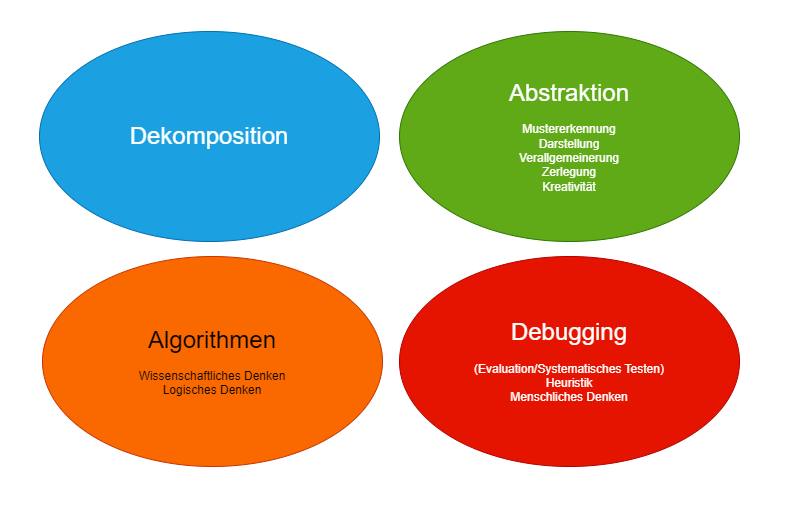
\includegraphics[width=1\linewidth]{Figures/CT}
    \caption{Die Haupt- und Unterkategorien Computational Thinking aus verschiedenen Forschungen, grafisch dargestellt}
\end{figure}

Zum Zweck der Forschung wird sich diese Arbeit auf die laut Schute vier häufigsten Aspekte von CT beschränken, die im ersten Abschnitt definiert wurden.

\subsection{Lerntypen}
Ebenso wie im Feld des CT, gibt es für Lerntypen kein allgemein akzeptiertes Modell. Allerdings gibt es einige Theorien die häufiger, besonders im Kontext von CS angewandt wird. Das bewährteste Modell hierbei ist das Felder-Silverman Lerntyp Modell (FSLSM) \cite{felder}. 
Das FSLSM wurde speziell im Kontext von hohen Abgangsraten in Studiengängen der Engineurswissenschaften untersucht, wird allerding auch vermehrt als Grundlage für Studien im Feld der Informatik verwendet \cite{kumar}.

\subsubsection{Differenzierung im Vergleich zu anderen Modellen}
Das FSLSM bezeichnet sich selbst als eine Studie, dessen Lernmodelle weder originell, noch allumfassend sind, und sich auf bereits existierende Modelle von etwa Jung \cite{jung}, Kolb \cite{kolb} und Briggs \cite{myers} beziehen.
Es muss zudem spezifiziert werden, dass Lerntypen nicht so eindeutig bestimmbar sind, wie es herkömmliche Modelle, zum Beispiel das weit verbreitete VARK Modell von N. Fleming implizieren mögen.
Beispielsweise nutzen alle Menschen sowohl fühlende als auch intuitive Fähigkeiten, bevorzugen allerdings tendenziell eine der beiden Methoden. Das Lernmodell setzt sich demnach nicht nach physisch festgelegten Merkmalen fest, sondern eher aus differenzierteren Präferenzen der Subjekte.

Das FSLSM beschreibt vier verschiedene Bereiche, in denen sich die Lernstile größtenteils unterscheiden \footnote{Ursprünglich als 5 Bereiche definiert, wobei die Dimension "Inductive Deductive" nachträglich aus dem Modell entfernt wurde. Als Grund hierfür wurde angegeben, dass die meisten Schüler und Studierende einen schlussfolgernden Stil zwar präferieren, aber induktive Methoden in den meisten Fällen laut der Ansicht der Autoren objektiv besser für das Verständnis der Lernenden sind \cite{felder}.}. Hierbei wird immer jeweils ein Gegensatzpaar beschrieben, in die sich Subjekte einsortieren lassen. Die meisten Personen präferieren demnach einer der beiden Stile jeder Kategorie.

% Kurze Zusammenfassung der Lerntypen
\begin{description}
    \item[Sensorisch und Intuitiv] Dieser Aspekt beschäftigt sich damit, wie Personen am besten die Welt um sich herum wahrnehmen können. Hierbei präferieren Personen gewöhnlich eine der beiden Methoden, auch wenn alle Menschen beide verwenden können. Sensorische Typen präferieren, Daten und Fakten auswendig zu lernen, und sich länger mit den Details eines Problemes zu beschäftigen. Sie ziehen es vor, einen klar erkennbaren Bezug auf die echte Welt zu haben, und Probleme mit etablierten Methoden zu lösen. Intuitive Typen hingegen können ihre Umgebung besser durch eigene Theorien, Vorstellungen und Vermutungen wahrnehmen, und setzen auf Innovation und Unsicherheiten. Sie sind besser darin, Abstraktion anzuwenden, und lernen neue Konzepte normalerweise schneller, als sensorisch veranlagte Personen.
    \item[Visuell und Auditiv] Dieser Aspekt beschäftigt sich mit der Art, wie Personen Input verarbeiten und Informationen am besten verstehen können. Visuelle Typen lernen am besten damit, was sie sehen können, etwa Diagramme, Bilder, Filme und Demonstrationen. Auditive Typen ziehen mehr aus Worten, sowohl geschriebenen als auch gesprochenen Erklärungen. Ihnen können besonders Gruppenarbeiten dabei helfen, das Material zu verstehen. Die Mehrheit der Lernenden sind typischerweise visuelle Lerner, was im Konflikt mit den typischen Stilen von Vorlesungen in den Bereichen Informatik und Ingenieurswissenschaften stehen. Hierbei wird meist ein frontaler Input gegeben.
    \item[Aktiv und Reflexiv]  Dieser Aspekt beschäftigt sich mit der Verarbeitung von Informationen zu Wissen. Aktive Lerner sind demnach besser darin, ihr Wissen direkt in der Anwendung zu vertiefen. Sie präfereieren Gruppenarbeiten, in denen sie sich aktiv einbringen können, und lernen mit herkömmlichen Vorlesungsstilen nicht so effektiv. Reflektive Lerner hingegen benötigen Zeit, um sich eigenständig mit Inhalten auseinanderzusetzen. Sie ziehen es vor, alleine zu arbeiten, und zuerst alle Fakten durchzudenken, bevor sie ein Problem angehen können.
    \item[Sequentiell und Global] Dieser Aspekt beschäftigt sich mit damit, wie Lernende Zusammenhänge verstehen. Sequentielle Lerner können besser in einer festgelegten logischen Reihenfolge arbeiten, etwa chronologisch mit einem Buch oder Inhalten einer Vorlesung. Globale Lerner hingegen stoßen meist auf Barrieren von Verständnis, und sind in dem Erlernen neuer Inhalte zunächst langsamer als sequentiell lernende Kommilitonen. Diese Lerner haben meist einen plötzlichen Moment des Verständnisses, in dem sich die globalen Zusammenhänge scheinbar schlagartig ergeben. Da die meisten Lehrformen sequentielle Lernstile stark zu begünstigen scheinen, ist es für die Unterstützung globaler Lerntypen wichtig, ein Bild des Großen und Ganzen zu Beginn eines Lerninhaltes zu bieten.
\end{description}

\subsection{Aktuelle Lerninhalte an Universitäten und Hochschulen}
Obwohl es immer mehr Studierende in der Informatik gibt, sind die Abbruchquoten in Deutschland dennoch immer noch vergleichsweise hoch \cite{dhzw}. Um die Frage zu beantworte, ob funktionale Programmierung Anfängern besser beim Erlernen von Programmierkenntnissen helfen kann, muss zunächst die Frage beantwortet werden, die der aktuelle Stand an deutschen Insititutionen ist.
Umfragen unter Entwicklern der letzten Jahre hat gezeigt, dass objektorientierte Sprachen noch immer zu den am meisten verwendeten zählen, sowohl im Berufsleben, als auch unter Lernenden \cite{stackoverflow}. Die Frage, die in diesem Abschnitt betrachtet werden soll, ist, ob auch an deutschen Universitäten noch vermehrt objektorientierte Paradigmen gelehrt werden.

\subsubsection{Übersicht bekannter Paradigmen}
Um die häufig behandelten Paradigmen untersuchen zu können, muss zuerst definiert werden, welche Kategorien es gibt. Hierzu werden die vier am häufigsten verbreiteten Paradigmen betrachtet \cite{normark}.

\begin{description}
    \item[Imperative Programmierung] Abfolge von Kommandos, die den Zustand des Programmes inkrementell ändern. Beschreibungen von Aktionen in einer geregelten Abfolge, etwa wie es bei einer Anleitung oder einem Rezept der Fall wäre.
    \item[Funktionale Programmierung] Orientierung an Funktionen aus mathematischer Sicht. Produzierte Werte sind unveränderlich, und das Programm hat keinen Zustand. Alle Operationen im Programm werden ausschließlich von Funktionen gehandhabt, und Funktionen werden als Objekte erster Klasse behandelt, so wie die Daten im Programm.
    \item[Logische Programmierung] Basiert auf Wahrheiten (Axiomen), Schlussregeln und Abfragen basierend auf sogenannten "Fakten".
    \item[Objektorientierte Programmierung] Modellierung von echten Objekten im Code. Daten und Funktionen werden in Objekten gekapselt, die wiederum in Klassen kategorisiert werden können. Klassen können in einer Hierarchie, etwa durch Konzepte wie Vererbung, organisiert werden.
\end{description}

\subsubsection{Untersuchung Curricula}\label{sec:curriculares}
Um zu untersuchen, wie verbreitet funktionale Programmierung momentan in Hochschulcurricula ist, wurden 121 Informatik Studiengänge an verschiedenen Universitäten und Hochschulen in Deutschland untersucht\footnote{Eine detaillierte Beschreibung des Vorgehen befindet sich im Anhang der Arbeit.}.
Hierbei ergab sich, dass die Mehrheit von Einführkursen der Informatik objektorientierte Programmierparadigmen behandeln.

\begin{figure}[h!]
    \centering
    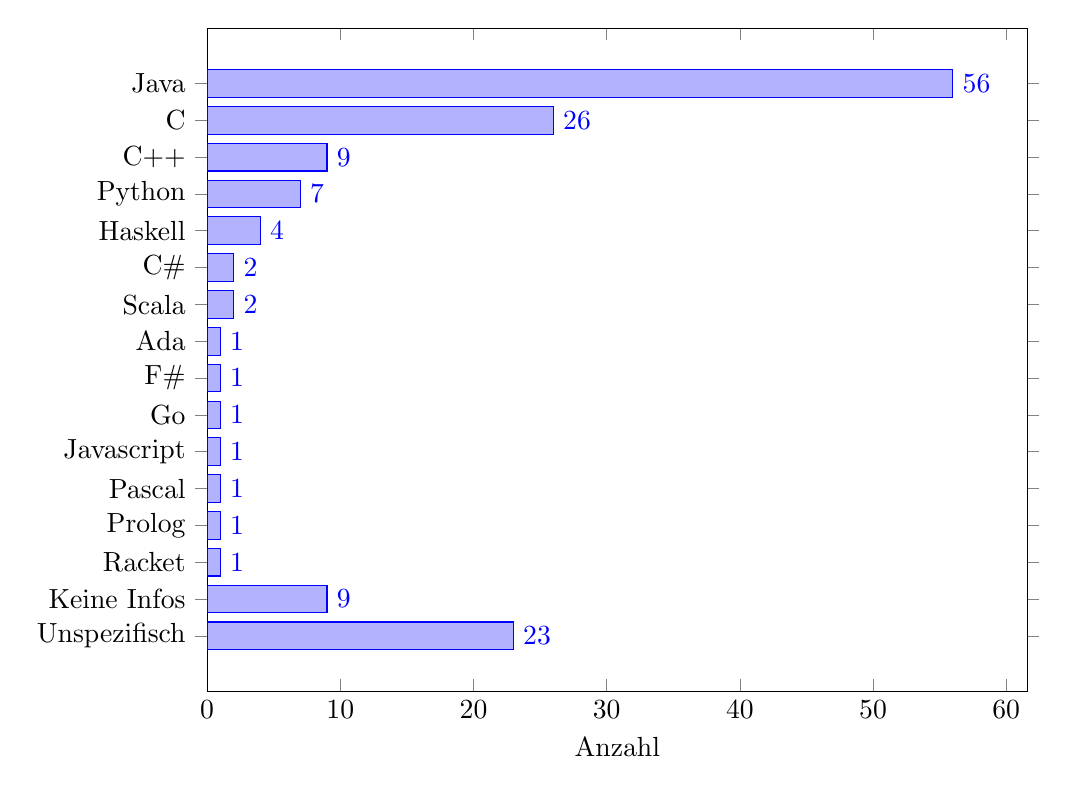
\begin{tikzpicture}
    \begin{axis}[
        xbar,
        width=12cm,
        height=10cm,
        symbolic y coords={{Unspezifisch}, {Keine Infos}, {Racket}, {Prolog}, {Pascal}, {Javascript}, {Go}, {F\#}, {Ada}, {Scala}, {C\#}, {Haskell}, {Python}, {C++},  {C}, {Java}},
        ytick=data,
        nodes near coords,
        xmin=0,
        xlabel={Anzahl}
    ]
        \addplot coordinates {
            (23,{Unspezifisch}) (9,{Keine Infos}) (1,{Racket}) (1,{Prolog}) (1,{Pascal}) (1,{Javascript}) (1,{Go}) (1,{F\#}) (1,{Ada}) (2,{Scala}) (2,{C\#}) (4,{Haskell}) (7,{Python})  (9,{C++}) (26,{C}) (56,{Java})
        };
    \end{axis}
\end{tikzpicture}

    \caption{Zahl der Programmiersprachen in Einführungskursen der Informatik}
\end{figure}

\begin{figure}[h!]
    \centering
    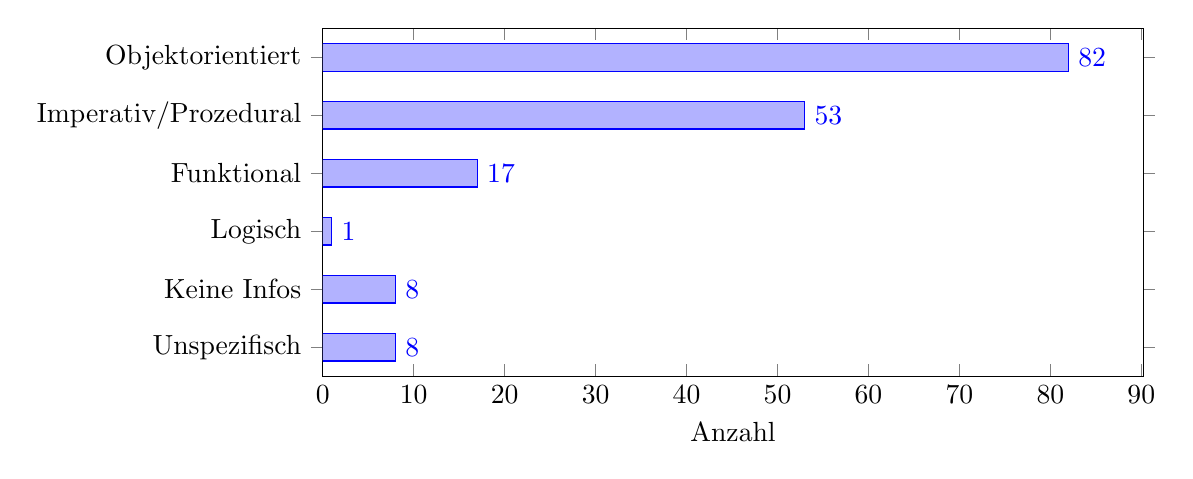
\begin{tikzpicture}
    \begin{axis}[
        xbar,
        width=12cm,
        height=6cm,
        symbolic y coords={{Unspezifisch}, {Keine Infos}, {Logisch}, {Funktional}, {Imperativ/Prozedural}, {Objektorientiert}},
        ytick=data,
        nodes near coords,
        xmin=0,
        xlabel={Anzahl}
    ]
        \addplot coordinates {
            (8,{Unspezifisch}) (8,{Keine Infos}) (1,{Logisch}) (17,{Funktional}) (53,{Imperativ/Prozedural}) (82,{Objektorientiert})
        };
    \end{axis}
\end{tikzpicture}
    \caption{Zahl der Paradigmen in Einführungskursen der Informatik}
\end{figure}

Wenn das funktionale Paradigma in den Modulzielen gelistet war, wurde meist nicht spezifiziert, welche Sprache verwendet wird, um das Konzept näher zu bringen, oder welche Ziele mit der Verwendung von funktionaler Programmierung speziell verfolgt werden.
In den meisten Fällen wird an Institutionen Java als Einführung in die Programmierung verwendet, und damit größtenteils imperative und objektorientierte Ansätze.
Es lässt sich also feststellen, dass ein funktionaler Ansatz für Programmieranfänger, zumindest in Deutschland, noch nicht praktisch ausprobiert wurde.